\documentclass[12pt]{article}
\usepackage{amsmath,mathtools}
\usepackage[usenames,dvipsnames]{xcolor}
%\usepackage[bitstream-charter]{mathdesign}
%\usepackage{mathptmx}

%\usepackage{textcomp}
%\usepackage{cmbright}
\usepackage[german]{babel}

%\usepackage[activate={true,nocompatibility},final,tracking=true,kerning=true,spacing=true,factor=1100,stretch=10,shrink=10]{microtype}

\usepackage[utf8]{inputenc}
\usepackage[T1]{fontenc}

\usepackage{libertine}
\usepackage{microtype}

\usepackage{siunitx}
\usepackage{fancyhdr}
\usepackage{sectsty}
\usepackage{setspace}
\usepackage{booktabs} % To thicken table lines
%\usepackage{chemstyle}
\usepackage[version=4]{mhchem}
\usepackage{graphicx}
\usepackage{tabularx}
%\usepackage[compatibility=4.7,language=german]{chemmacros}

\usepackage[ddmmyyyy]{datetime}
\renewcommand{\dateseparator}{.}
\usepackage{overcite}
\renewcommand\citeform[1]{[#1]}

\sectionfont{\fontsize{12}{15}\selectfont}
\pagestyle{fancy}

\cfoot{\thepage}

\lhead{Nevroz Arslan }
\rhead{\today}
\setlength{\headheight}{15pt}
 \sisetup{
        detect-all %,               %% Benutze gleiche Schriftarten wie im Text
    }
\renewcommand{\thesection}{\arabic{section}.}
\renewcommand{\thesubsection}{\thesection\arabic{subsection}}
\renewcommand{\headrulewidth}{0pt}
\renewcommand{\familydefault}{\sfdefault} 
\begin{document}

\begin{onehalfspace}
  {\hfil  \textbf{\large Darstellung von Bis($\eta^5$-cyclopentadienyl)eisen}\hfil}
\par
  \vspace{1cm}
\hfil \textbf{Präparat Nr. 1 von 4 }\hfil
\section{Reaktionstyp: \textnormal{1. Reduktion 2. Komplexierung}  }
\begin{figure}[!ht]
   \centering
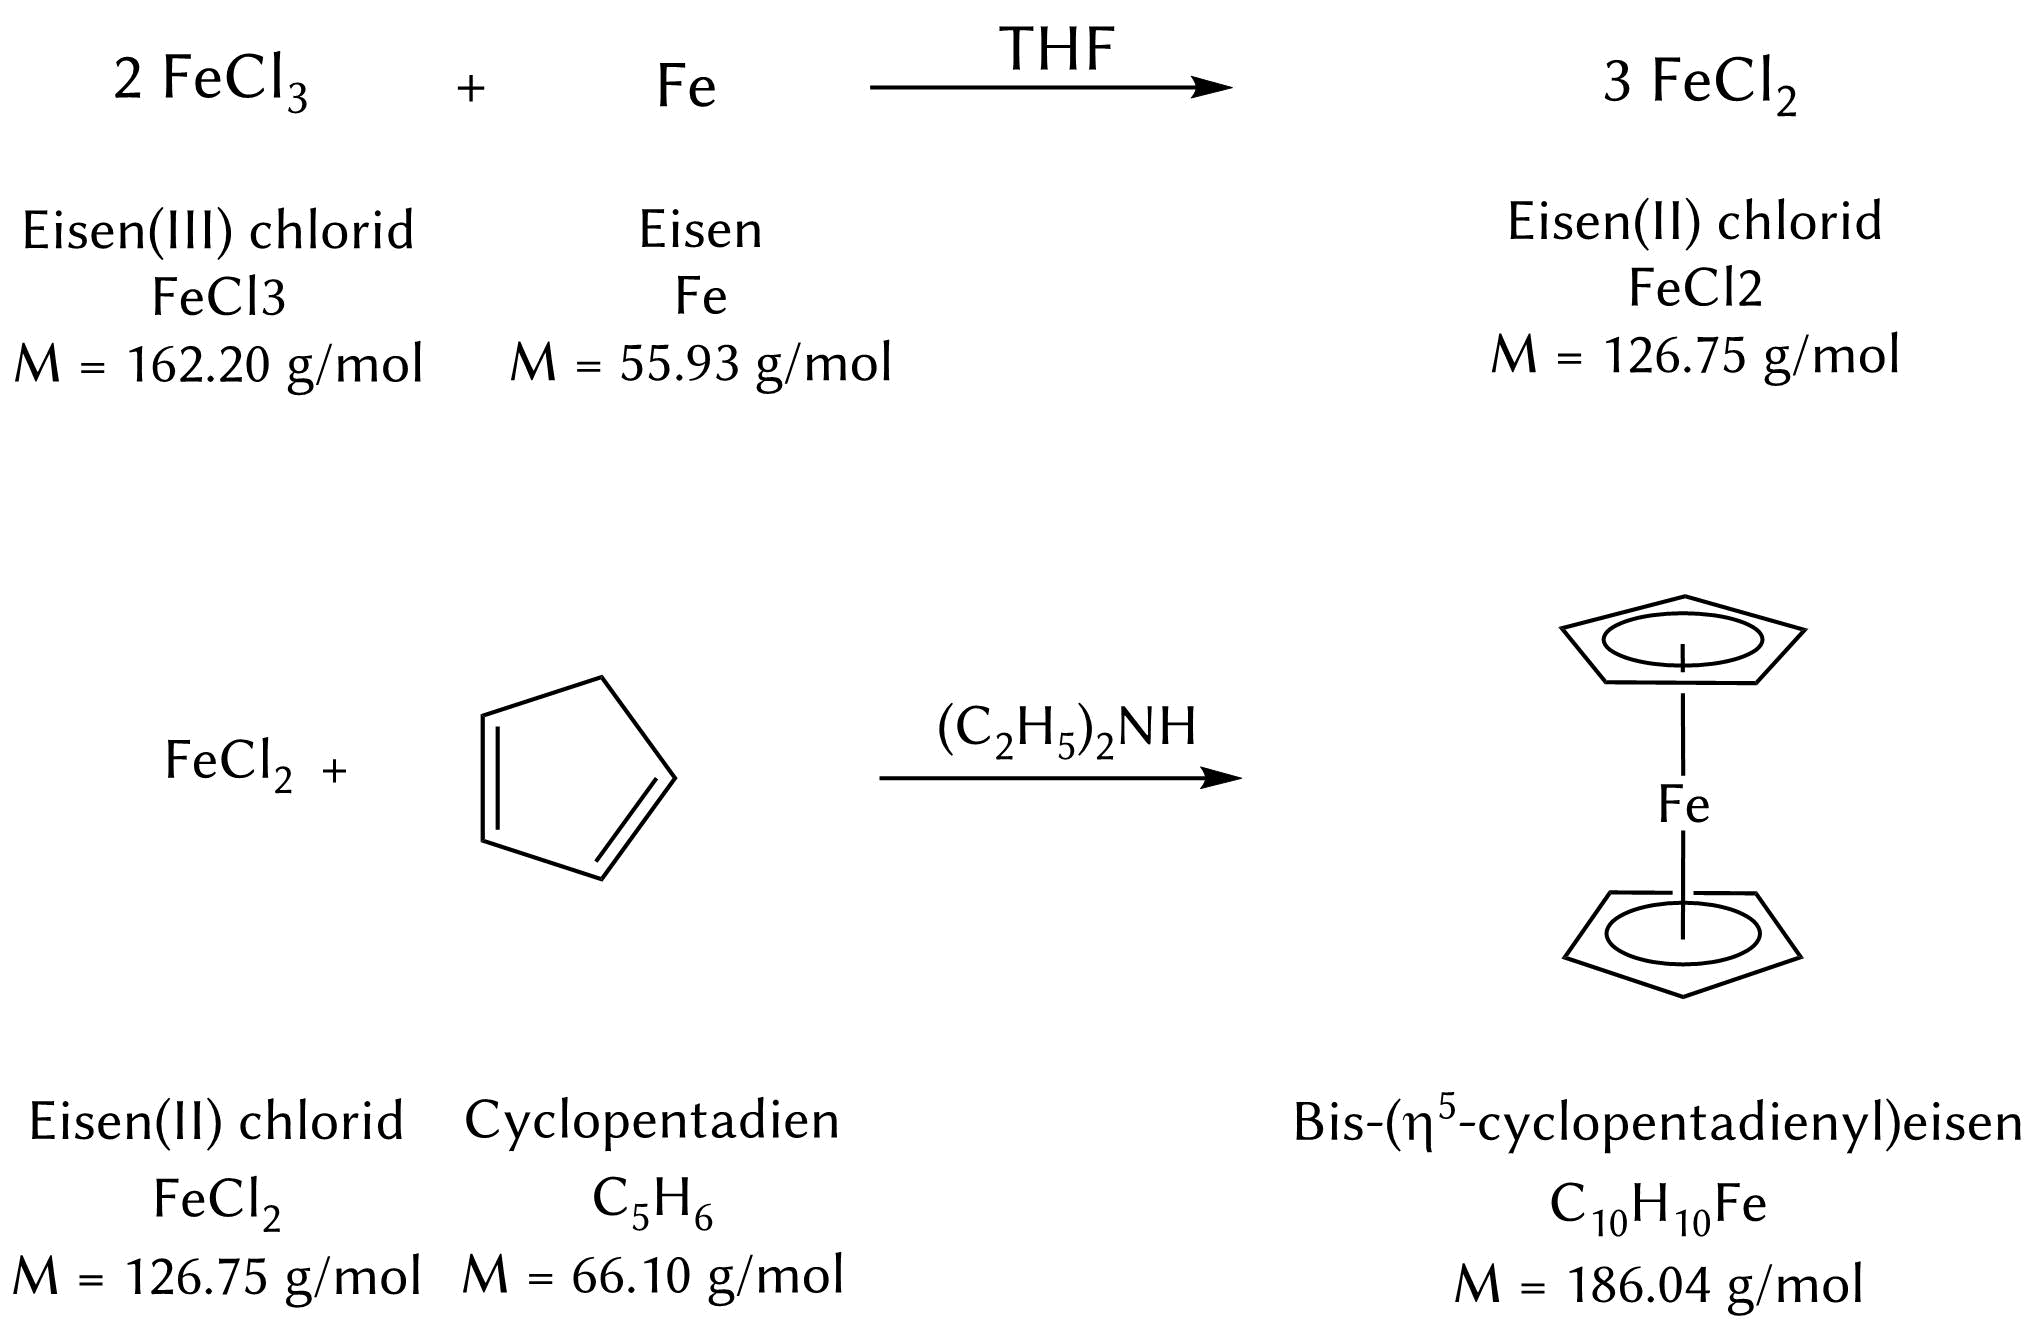
\includegraphics[width=\textwidth]{reaktion.png}
\end{figure}

\section{Berechnung des Ansatzes: }
Es sollten aus 9.430 g (58.21 \si{\milli\mol}) Eisen(III) Chlorid Bis($\eta^5$-cyclopentadienyl)eisen hergestellt werden.
Die Umrechnung des Literaturansatzes\cite{bio} ergab folgenden Ansatz:\\
\begin{tabularx}{\textwidth}{lrrrr}
\toprule
\textbf{Bezeichnung} &\textbf{ M [\si{\gram\per\mol}]} & \textbf{n [\si{\milli\mol}]} & \textbf{Menge} & \textbf{Equiv}\\
\midrule
Eisen(III) Chlorid     & 162.20  & 58.21  & 9.430 g  &  2.00  \\
Eisen        & 55.93   & 29.10  & 1.620 g  &  1.00 \\
Cyclopentadien      & 66.10   & 174.60  & 11.54 \si{\gram} &  6.00 \\
Diethylamin & 73.14   & 349.20  & 25.54 \si{\gram} &  12.00\\
Tetrahydrofuran  &   &  &  &  LM\\
\bottomrule
\end{tabularx}\\

\normalsize \section{Durchführung \cite{bio}}
In einem ausgeheizten 250 ml-Dreihalskolben wurden unter Schutzgas \ce{FeCl_3} (9.43 \si{\gram}, (58.21 \si{\milli\mol})) und \ce{Fe} (1.62 \si{\gram}, 19.40 \si{\milli\mol}) in Tetrahydrofuran (50 \si{\milli\liter}) suspendiert. Diese Suspension wurde 5 Stunden lang unter Rückfluss erhitzt. Danach wurde das Lösungsmittel am Hochvakuum abgezogen. Der Rückstand wurde hintereinander mit Cyclopentadien (11.54 \si{\gram}, 174.60 \si{\milli\mol}) und Diethylamin(25.54 \si{\gram}, 349.20 \si{\milli\mol}) unter Kühlung mit einer Eis-Wasser-Kältemischung versetzt. Das Reaktionsgemisch wurde noch 8 Stunden bei der Raumtemperatur gerührt und anschließend durch Kältedestillation zur Trockne eingedampft. Danach wurde der Rückstand in einer Soxhlet-Apparatur mit Petrolether extrahiert. Der so erhaltene Auszug wurde über Nacht in der Gefriertruhe auskristallisieren gelassen. Das Produkt wurde als orangener Feststoff (5.704 \si{\gram}, 11.36 \si{\milli\mol}, 35 \%) erhalten.\\
\noindent
\textbf{Thermisches Cracken von Dicyclopentadien:}\\
In einem 50 ml-Schlenkkolben wurden Dicyclopentadien (11.54 \si{\gram}, 87.30 \si{\milli\mol}) mit einer Vigreux-Kolonne in eine eisgekühlte Vorlage destilliert. \\
\noindent
\textbf{Trocknen des Lösungsmittels:}\\
\noindent
In einem 500 ml-Rundkolben wurden Tetrahydrofuran (250 \si{\milli\liter}) vorgelegt.
Danach wurde Natrium mit Hilfe einer Natriumpresse als dünner Draht in das Lösungsmittel eingebracht. 
Zur Überprüfung der Wasserfreiheit wurde Benzophenon hinzugegeben. Der Kolben wurde anschließend mit einem Rückflusskühler ausgestattet und unter Schutzgas erhitzt. Die Trocknung mit Natrium wurde solange fortgesetzt, bis sich Benzophenon die typische Blaufärbung zeigt.
\section{Ausbeute}
\begin{tabular}{ rl}
  16.240 g (87.31 \si{\milli\mol}) =  & 100 \%\\
  5.704 g (11.36 \si{\milli\mol}) =  & 35 \% (Lit.\cite{bio} : 66 \%) \\
 \end{tabular}
\section{Spektrenauswertung}

\begin{figure}[!htbp]
   \centering
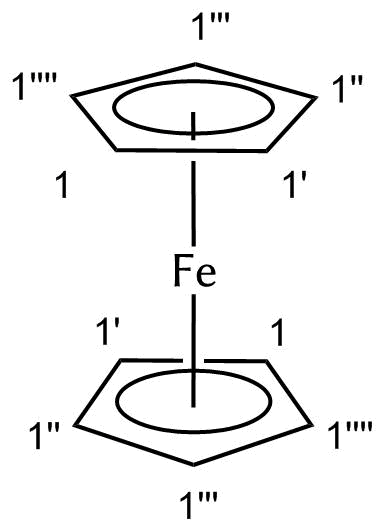
\includegraphics[scale=0.4]{auswert.png}
\end{figure}
\noindent
\textbf{\ce{^1_{}H-NMR}} (300 MHz, \ce{CDCl_3}): \ce{$\delta$} = 4.12 (s, 10 H, 1-H) ppm.
\section{Mechanismus\cite{wiberg}}
Die Reaktion läuft in zwei Schritten ab.
Im ersten Schritt der Reaktion erfolgt eine Komproportinierung. Durch gleichzeitige Reduktion des Eisen(III)-Chlorids (\textbf{1})
und Oxidation des Eisens (\textbf{2}) bildet sich Eisen(II)-Chlorid Eisens (\textbf{3}).
Im zweiten Schritt der Reaktion erfolgt eine Substitution. Dazu wird Cyclopentadien (\textbf{4}) durch eine starke Base in Cyclopentadienylanion \textbf{5} überführt. Anschließend greift Das Cyclopentadienylanion das Eisen des Eisen(III)-Chlorids (\textbf{1}) an. 
Unter Abspaltung von Chloridionen entsteht das gewünschte Produkt Bis($\eta^5$-cyclopentadienyl)eisen (\textbf{6}).
\begin{figure}[!ht]
   \centering
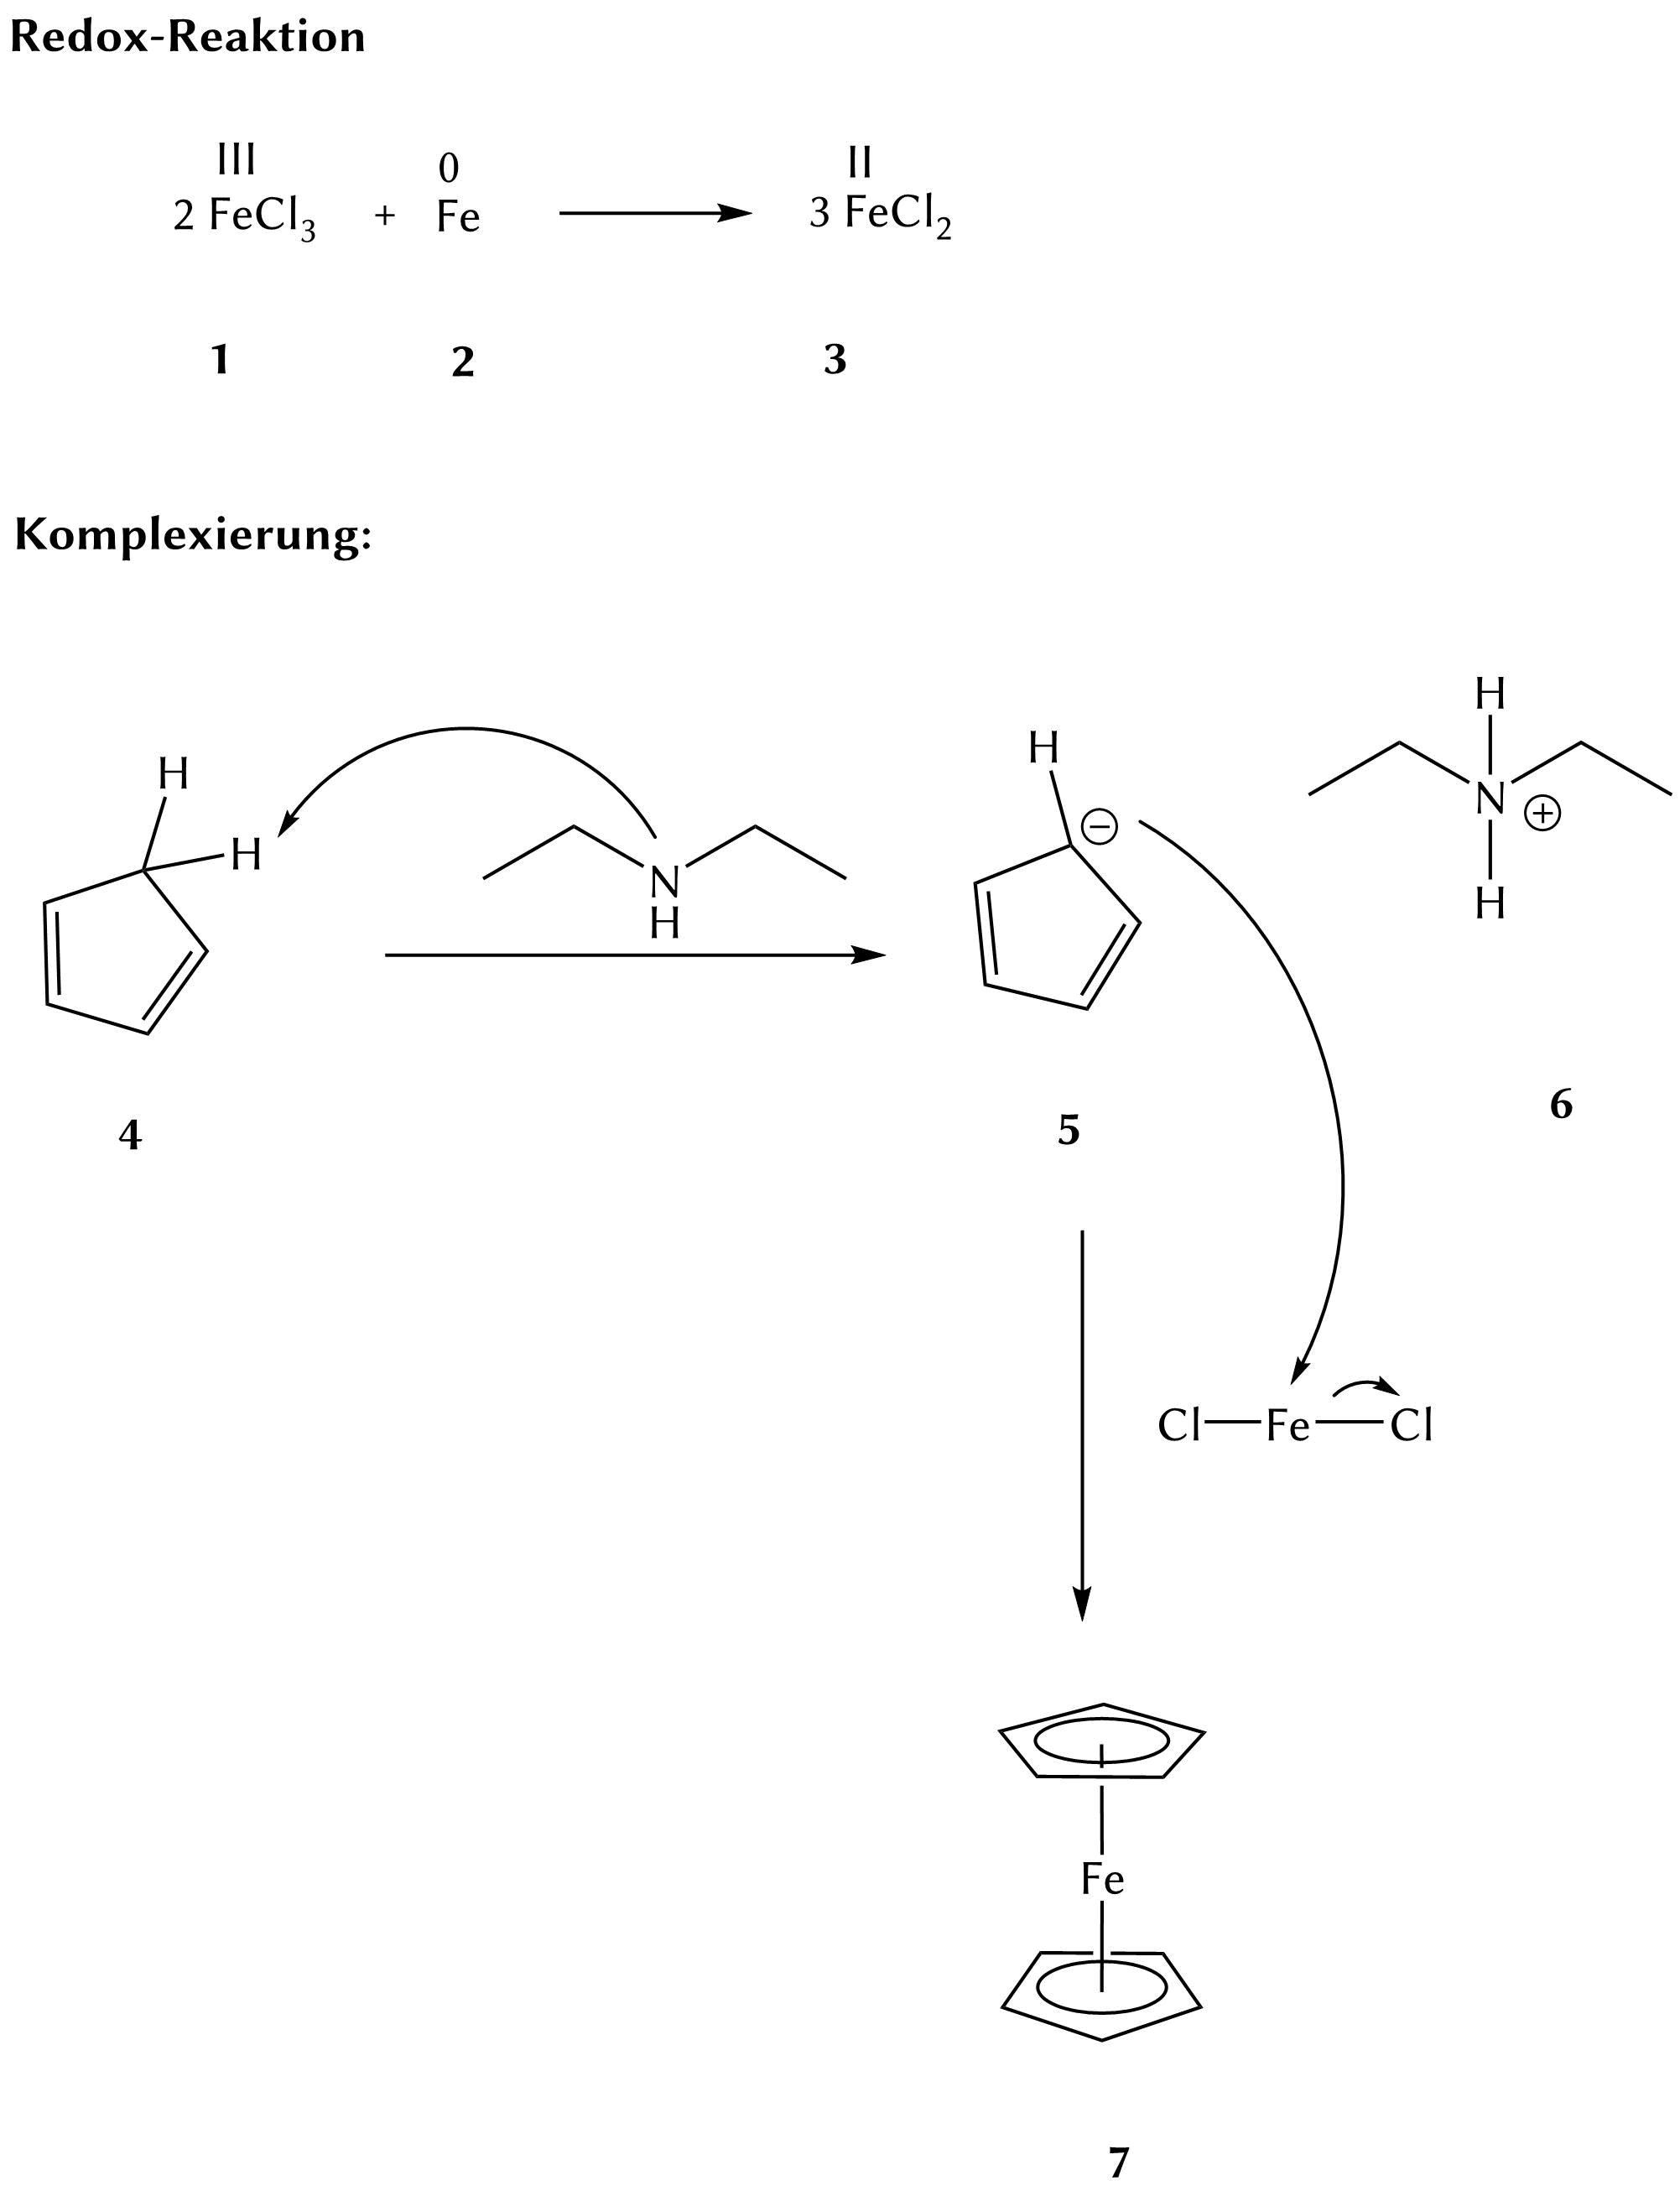
\includegraphics[width=\textwidth]{mechan.png}
\end{figure}
\section{Abfallentsorgung}
Das im Rotationsverdampfer abgetrennte Lösungsmittel wurde im Behälter für halogenfreie Kohlenwasserstoffe entsorgt.
Der Rest des Natriums, das von dem Trocknen des Lösungsmittels übriggeblieben war, wurde mit Ethanol zerstört. 
\section{Literatur}
\renewcommand{\section}[2]{}%
\begin{thebibliography}{}
\bibitem{bio}
G. Brauer, \textit{Handbuch der Präpativen Anorganischen Chemie Band III.}, 3. Aufl., Ferdinand Enke Verlag, Stuttgart \textbf{1981}, S. 1842.
\bibitem{wiberg}
A. F. Holleman, N. Wiberg \textit{Lehrbuch der Anorganischen Chemie}, 3. Aufl., de Gruyter, Berlin \textbf{2007}, S. 1855.
\end{thebibliography}
\end{onehalfspace}
\end{document}